\section{Communication Architecture}

Services communicate synchronously over REST only when the caller needs the
answer to continue, and asynchronously through a message broker for everything
else. All synchronous calls have timeouts, bounded retries with backoff,
idempotency keys where they change state, and correlation IDs. All events share
one envelope (\texttt{eventId}, \texttt{eventType}, \texttt{eventVersion},
\texttt{occurredAt}, \texttt{producer}, \texttt{correlationId},
\texttt{causationId}, payload), are published through the outbox, delivered at
least once and deduplicated by consumers on (\texttt{eventId},
\texttt{consumer}), with a dead-letter queue for poison messages.

Three failure behaviours are common to every work stream: if the broker is
down, events wait in the outbox and synchronous operations continue; duplicate
events are ignored; and if the Audit Service is down, sensitive actions are
rejected (fail closed) while the rest of the system keeps working.

\subsection{Synchronous Communication}

\begin{itemize}
  \item \textbf{Payments.} The Reservation Service waits for the payment
    authorization ($\approx$1\,s timeout) because the guest needs to know if
    the money was held. Refund requests only wait for acceptance
    (\texttt{202}); the refund is processed asynchronously. Gateway calls
    always reuse the same idempotency key on retries.
  \item \textbf{Reservation.} The guest gets the hold immediately
    (\texttt{201} or \texttt{409}); the host gets the effective rate when
    saving a listing (Pricing timeout $\approx$500\,ms, one retry within
    1.5\,s). Pricing is never on the booking path.
  \item \textbf{Pricing.} Besides the multiplier request, the daily occupancy
    query and the monthly SerpAPI call are synchronous batch calls outside any
    user request; their failure only delays indicators.
  \item \textbf{Identity.} Tokens are validated locally with cached public
    keys ($<$5\,ms), so there is no identity call per request. Login checks
    role and status in User Profile (cached 60\,s, fails closed). Messages are
    stored before the sender gets the answer.
\end{itemize}

\begin{figure}[H]
  \centering
  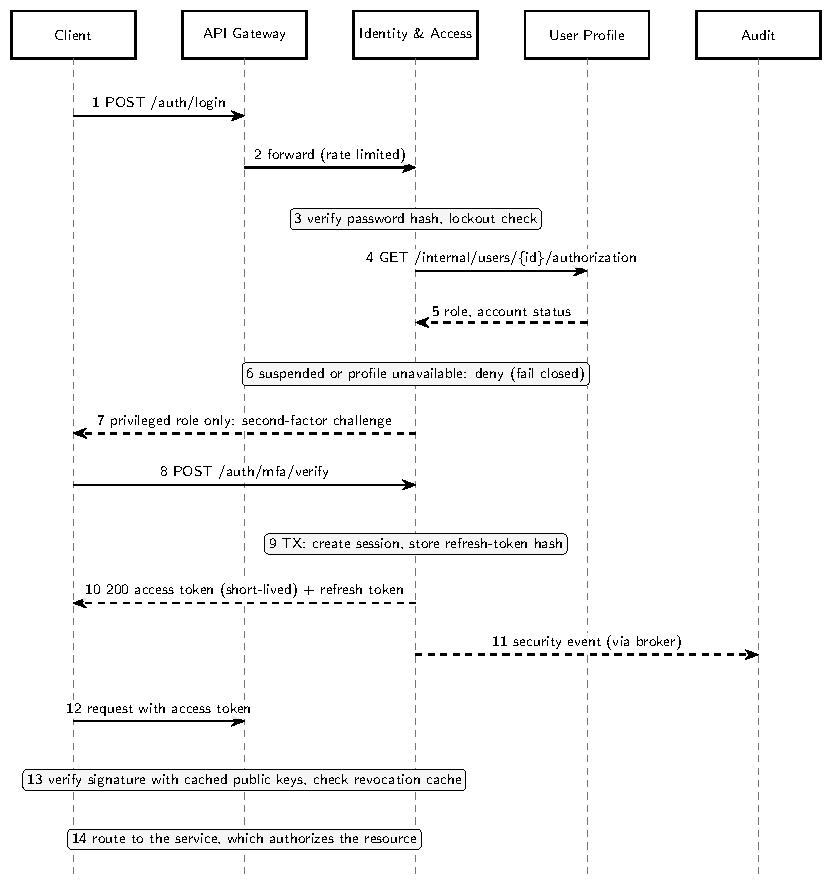
\includegraphics[width=\linewidth]{images/identity_auth_sequence.pdf}
  \caption{Log In with MFA for privileged roles and local token validation.}
  \label{fig:id-auth}
\end{figure}

\begin{figure}[H]
  \centering
  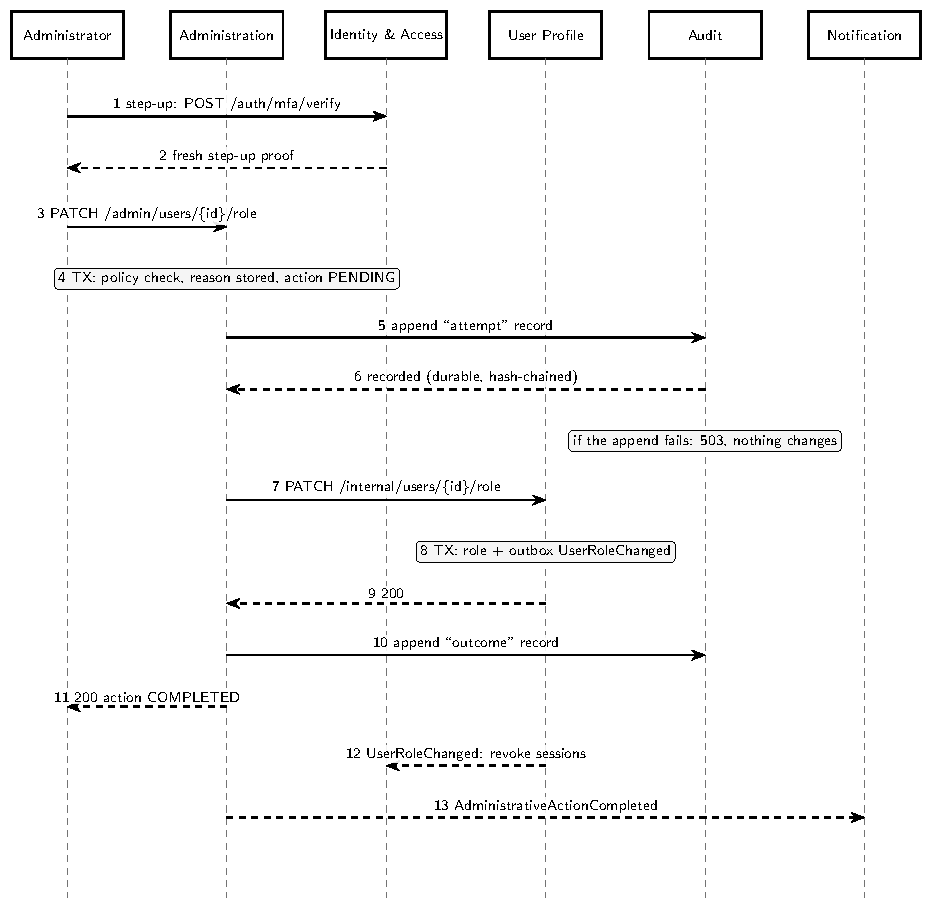
\includegraphics[width=\linewidth]{images/identity_admin_sequence.pdf}
  \caption{Manage Users: step-up MFA, audit before effect, delegation and
  session revocation.}
  \label{fig:id-admin}
\end{figure}

\subsection{Asynchronous Communication}

Events are used for work that must not delay or fail the user's operation.
Table~\ref{tab:events} lists the main events.

\begin{longtable}{@{}L{4.2cm}L{2.5cm}L{3.0cm}L{4.1cm}@{}}
\toprule
\textbf{Event} & \textbf{Producer} & \textbf{Consumers} & \textbf{Purpose} \\
\midrule
\endhead
\texttt{PaymentSucceeded}, \texttt{PaymentFailed} & Payment Coord. &
  Reservation, Notification & Confirm the reservation or release dates. \\
\texttt{PaymentCaptured}, \texttt{PaymentVoided} & Payment Coord. &
  Ledger, Audit & Write the journal entry. \\
\texttt{Refund\allowbreak Status\allowbreak Changed} & Payment Coord. & Ledger, Support,
  Notification, Audit & Refund requested, succeeded or failed. \\
\texttt{Payout\allowbreak Status\allowbreak Changed} & Ledger & Notification, Audit & Host payout
  status. \\
\texttt{ReservationHeld}, \texttt{Confirmed}, \texttt{Cancelled},
  \texttt{Expired} & Reservation & Payment Coord., Ledger, Notification &
  Capture, void or refund; schedule payout; inform users. \\
\texttt{ListingCreated}, \texttt{Updated}, \texttt{Deactivated},
  \texttt{Availability\allowbreak Changed} & Reservation & Search & Refresh the search
  index. \\
\texttt{Reservation\allowbreak Flagged}, \texttt{Admin\allowbreak Action\allowbreak Recorded} & Reservation &
  Support, Administration & Review reservations of a paused listing. \\
\texttt{HoldExpired} & Scheduler & Reservation & Release the hold. \\
Search events & Search & Demand Indicators & Count searches per zone. \\
\texttt{Demand\allowbreak Indicators\allowbreak Updated}, \texttt{Context\allowbreak Indicators\allowbreak Updated} &
  Demand, Context & Pricing & Refresh the zone snapshot. \\
\texttt{UserRegistered} & Identity \& Access & Profile, Notification,
  Audit & Create the profile, welcome message. \\
\texttt{UserRoleChanged} & User Profile & Identity, Notification, Audit &
  Revoke sessions, notify, record. \\
\texttt{MessageCreated} & Messaging & Notification & New-message alert (IDs
  only). \\
\texttt{Support\allowbreak Case\allowbreak Created}, \texttt{Updated} & Support & Notification,
  Audit & Inform the reporter, record transitions. \\
\texttt{Administrative\allowbreak Action\allowbreak Completed} & Administration & Audit,
  Notification & Record the outcome, notify the user. \\
\bottomrule
\caption{Main events.}
\label{tab:events}
\end{longtable}

\paragraph{Why these interactions are asynchronous.}
\begin{itemize}
  \item \textbf{Payment results:} 3-D Secure and slow methods finish minutes
    after the request; the 10-minute hold covers that time. Gateway refunds
    can take days, so they are accepted at once and reported by event.
  \item \textbf{Ledger:} if a capture waited for the ledger, two services at
    99.9\,\% in a chain would give about 99.8\,\% booking availability.
  \item \textbf{Pricing indicators:} searches are 60\,\% of the traffic and
    must not call the engine; calling three services and an external API
    inside a 500\,ms listing save would make it fragile.
  \item \textbf{Notifications:} an email, push or SMS failure must never fail
    a payment, a message, a case or an administrative change.
  \item \textbf{Role changes:} propagating them synchronously would be a
    distributed transaction; events plus short token lifetimes and revocation
    are enough.
\end{itemize}

\paragraph{Notification delivery.} Each notification has the key
\texttt{(eventId, userId, channel)}, inserted with the outbound task, so
repeated deliveries are discarded. Transient errors are retried with
exponential backoff and jitter, permanent ones (invalid address, withdrawn
consent) are not; if push fails, email is tried when consented; exhausted
tasks go to the dead-letter queue for replay.

\paragraph{Work-stream specific failures.}
\begin{longtable}{@{}L{4.6cm}L{9.2cm}@{}}
\toprule
\textbf{Failure} & \textbf{Behaviour} \\
\midrule
\endhead
Gateway does not answer in time & Payment stays \texttt{PENDING}, never
  assumed failed; resolved by webhook or reconciler with the same key. \\
Hold expires while payment pending & \texttt{Reservation\allowbreak Expired} voids the
  authorization. \\
Gateway rejects a refund & Cancellation stands; a support case is opened. \\
Pricing Service down & Listing save returns \texttt{502} and the host
  retries; bookings are unaffected. \\
Zone without snapshot; indicators stale & \texttt{STANDARD} with
  \texttt{fallback = true}; otherwise the last snapshot is used. \\
SerpAPI unavailable & Monthly run retried; previous context kept. \\
Notification provider fails & Source operation unaffected; retries,
  fallback channel, dead-letter queue. \\
Message recipient offline & Message stored; push sent; history read on
  reconnect, duplicates discarded by \texttt{messageId}. \\
\bottomrule
\caption{Failure scenarios specific to each work stream.}
\label{tab:failures}
\end{longtable}

\begin{figure}[H]
  \centering
  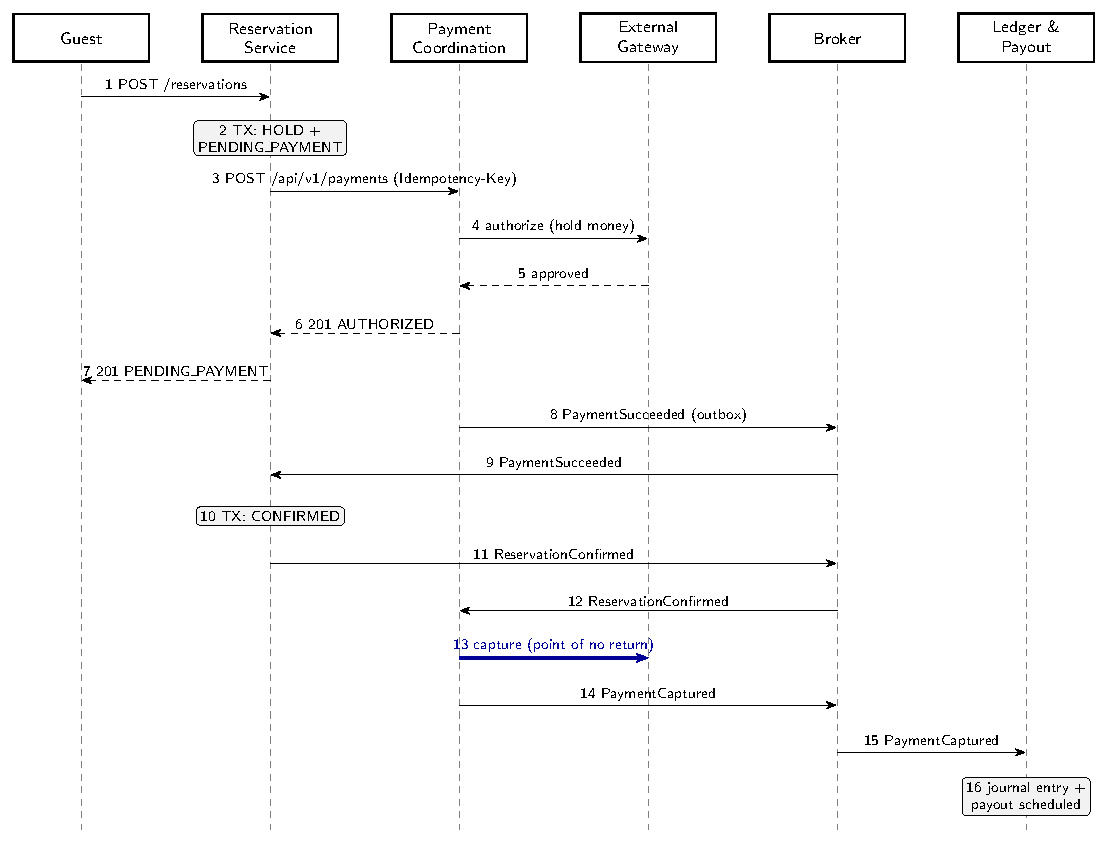
\includegraphics[width=\linewidth]{images/payments_booking_sequence.pdf}
  \caption{Booking with payment, capture and accounting.}
  \label{fig:pay-booking}
\end{figure}

\begin{figure}[H]
  \centering
  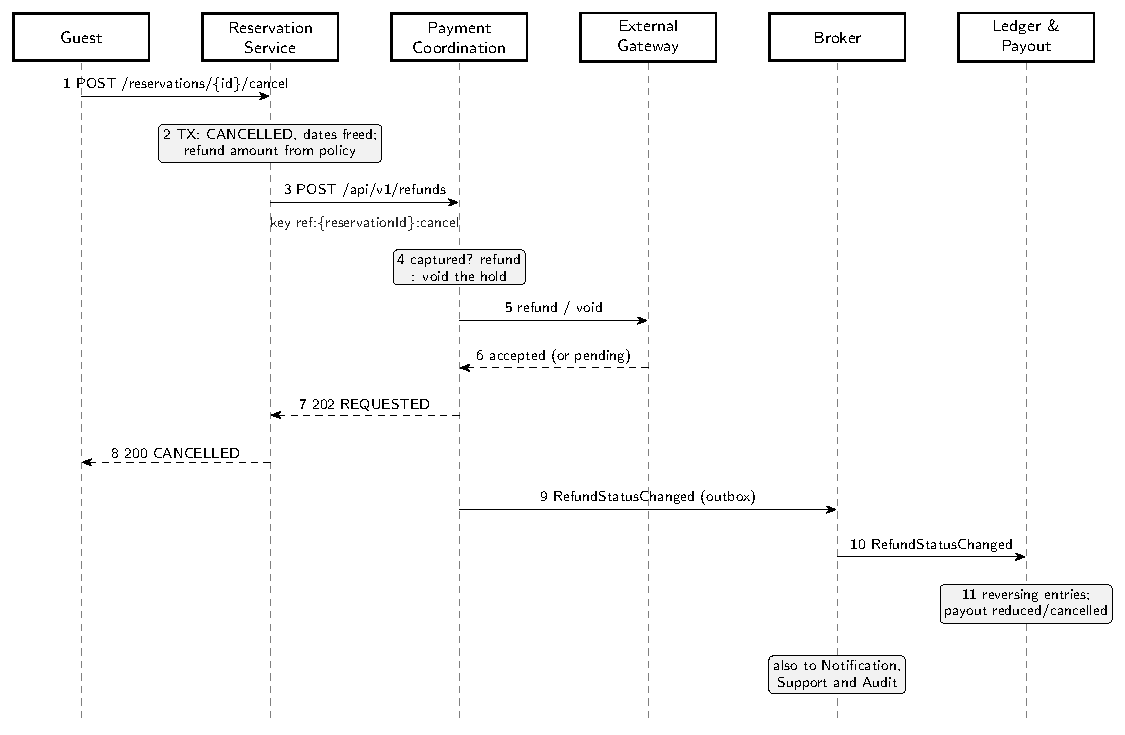
\includegraphics[width=\linewidth]{images/payments_cancel_sequence.pdf}
  \caption{Cancel Reservation: void if not captured, refund otherwise.}
  \label{fig:pay-cancel}
\end{figure}

\begin{figure}[H]
  \centering
  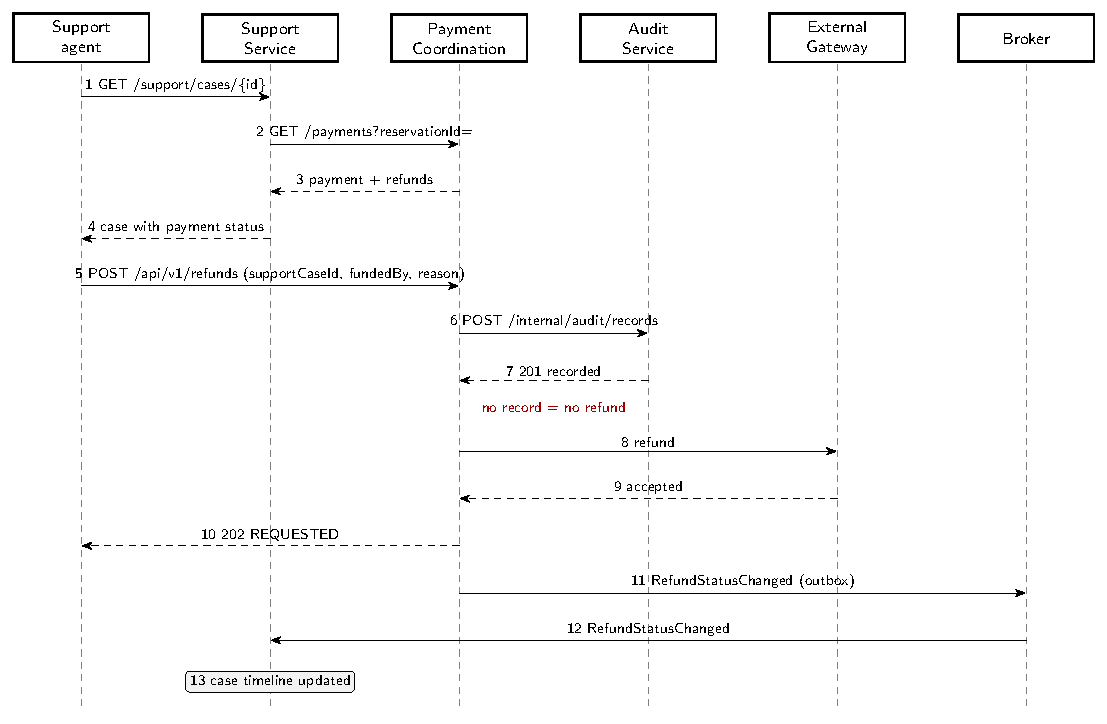
\includegraphics[width=\linewidth]{images/payments_manual_refund_sequence.pdf}
  \caption{Handle Refunds: manual refund audited before effect.}
  \label{fig:pay-manual}
\end{figure}

\begin{figure}[H]
  \centering
  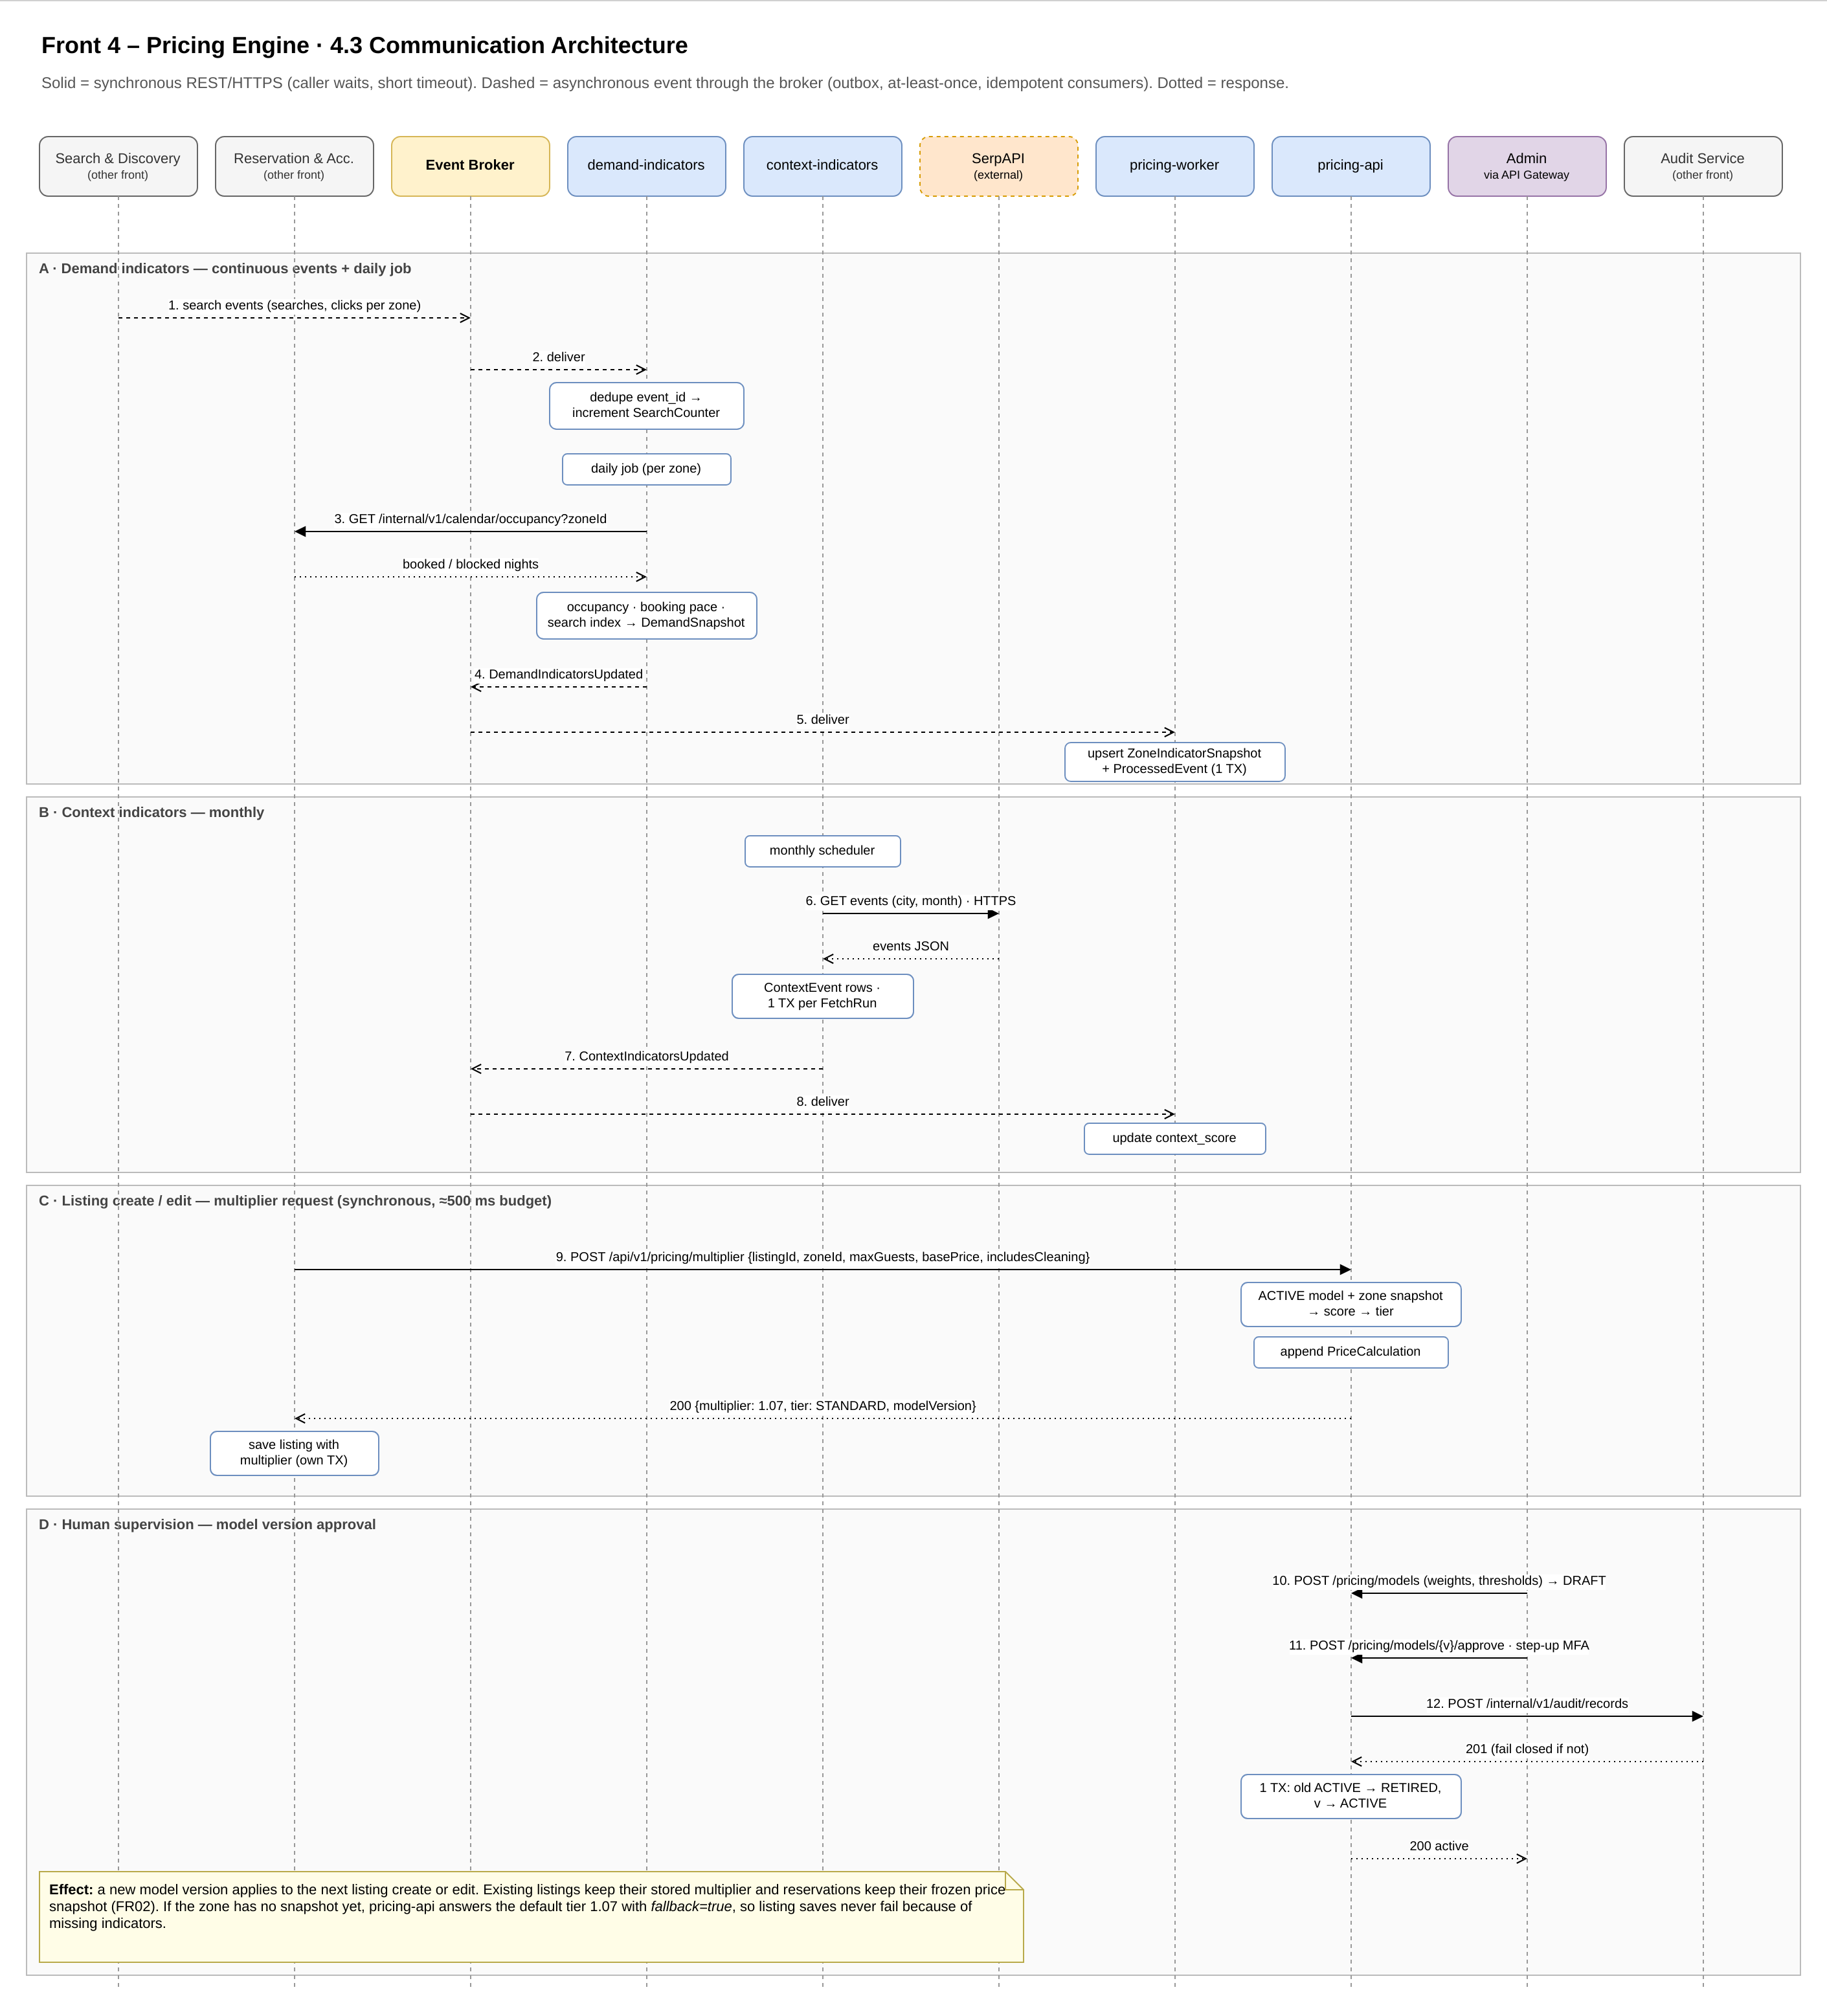
\includegraphics[width=\linewidth]{images/pricing_43_communication.png}
  \caption{Pricing Engine flows: (A) demand indicators, (B) monthly context,
  (C) multiplier request, (D) model approval.}
  \label{fig:price-sequence}
\end{figure}

\begin{figure}[H]
  \centering
  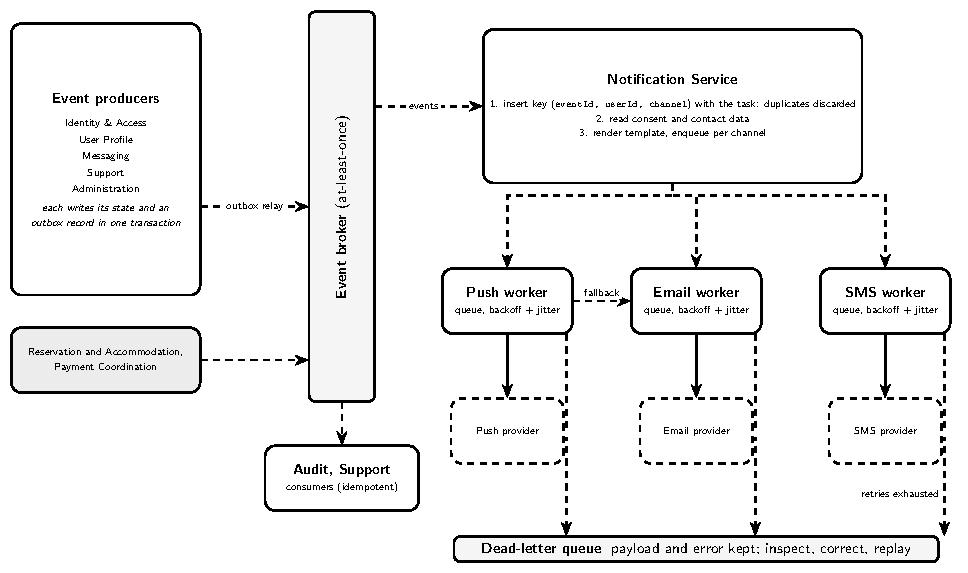
\includegraphics[width=\linewidth]{images/identity_event_flow.pdf}
  \caption{Event flow and notification pipeline.}
  \label{fig:id-events}
\end{figure}

\begin{figure}[H]
  \centering
  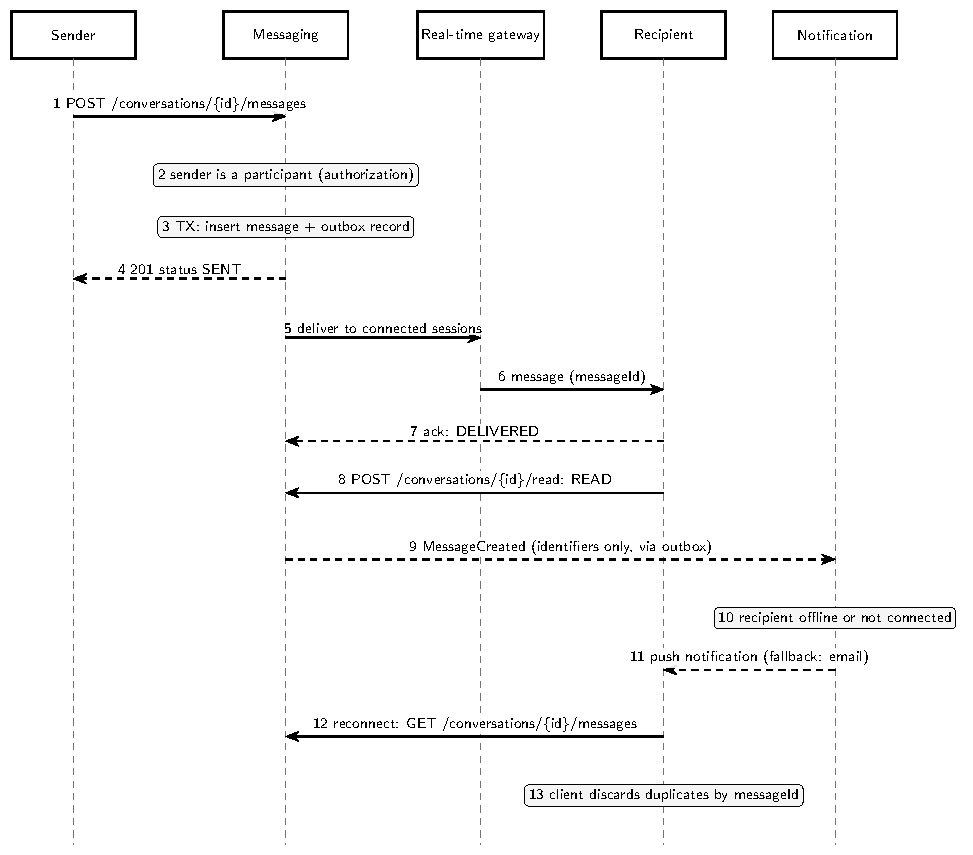
\includegraphics[width=\linewidth]{images/identity_message_sequence.pdf}
  \caption{Communicate with Host or Guest: store first, then deliver in real
  time or by push.}
  \label{fig:id-message}
\end{figure}

\subsection{Communication Matrix}

Table~\ref{tab:matrix} consolidates all interactions; each one appears once.

\begin{longtable}{@{}L{2.5cm}L{2.5cm}L{3.9cm}L{1.6cm}L{2.6cm}@{}}
\toprule
\textbf{From} & \textbf{To} & \textbf{Operation or event} & \textbf{Pattern} & \textbf{Latency / guarantee} \\
\midrule
\endhead
\multicolumn{5}{@{}l}{\emph{Synchronous}} \\
Client (via Gateway) & Reservation & Listings, blocks, reservations,
  agreements & REST & p95 1.5\,s \\
Reservation & Pricing & Multiplier on listing create or edit & REST &
  p95 150\,ms; timeout 500\,ms \\
Reservation & Payment Coord. & Payment intent & REST & p95 $\leq$ 1\,s;
  idempotent \\
Reservation, support agent & Payment Coord. & Refund request & REST (accept) &
  p95 300\,ms \\
Support & Reservation, Payment Coord. & Case context, refund status & REST &
  p95 300\,ms \\
Demand Indicators & Reservation & Calendar occupancy (daily) & REST &
  Batch; retries \\
Context Indicators & SerpAPI & Events by city and month & HTTPS & Monthly;
  retries \\
Payment Coord., Ledger & Gateway & Authorize, capture, void, refund, payout &
  HTTPS & Same key on retry \\
Admin, analyst & Pricing & Model versions, history & REST & p95 300\,ms \\
Client & Identity \& Access & Login, refresh & REST & p95 300 / 100\,ms \\
Gateway, services & Identity keys & Token validation & Local & $<$5\,ms \\
Identity \& Access & User Profile & Role and status at login & REST & p95
  100\,ms; fails closed \\
Client & Messaging & Send, history; real time & REST + WS & p95 200 /
  150\,ms \\
Messaging, Notification & User Profile & Display and contact data & REST &
  p95 150\,ms; cached \\
Administration & User Profile, Reservation & Role change, listing pause &
  REST & p95 300\,ms \\
Payments, Pricing, Admin., Identity, Support & Audit & Append a record &
  REST & p95 150\,ms; fails closed \\
Auditor & Audit & Query records, proofs & REST & Read-only \\
\addlinespace
\multicolumn{5}{@{}l}{\emph{Asynchronous}} \\
Gateway & Payment Coord. & Webhooks & HTTPS & Signed; inbox dedup \\
Payment Coord. & Reservation & \texttt{PaymentSucceeded},
  \texttt{PaymentFailed} & Event & At-least-once \\
Reservation & Payment Coord., Ledger & Reservation lifecycle & Event &
  At-least-once \\
Payment Coord. & Ledger & \texttt{PaymentCaptured},
  \texttt{Refund\allowbreak Status\allowbreak Changed} & Event & One entry per event \\
Scheduler & Reservation & \texttt{HoldExpired} & Message & At-least-once \\
Reservation & Search & Listing and availability events & Event &
  At-least-once \\
Search & Demand Indicators & Search events & Event & At-least-once \\
Demand, Context & Pricing & Indicator updates & Event & At-least-once \\
Any producer & Notification, Audit, Support & Domain events & Event &
  Backoff; dead-letter queue \\
Notification & Providers & Email, push, SMS & Queue + API & Fallback;
  dead-letter queue \\
Audit & Search index & \texttt{Audit\allowbreak Record\allowbreak Appended} & Event & Eventual;
  rebuildable \\
\bottomrule
\caption{Communication matrix.}
\label{tab:matrix}
\end{longtable}
